% \documentclass[acmsmall, natbib=true]{acmart}
\documentclass[sigconf, natbib=true]{acmart}
\usepackage{float}
\usepackage{booktabs} % For formal tables
\usepackage{url}
\usepackage{color}
\usepackage{enumitem}
\usepackage{multirow}
\hyphenation{Media-Eval}
\usepackage[toc,page]{appendix}
\usepackage{rotating,multirow}
% DOI
\acmDOI{}

% ISBN
\acmISBN{}

\settopmatter{printacmref=false}

\setlength{\tabcolsep}{3pt}
\renewcommand{\arraystretch}{1}
\acmConference[IR'23-'24]{Information Retrieval}{Radboud University}{Nijmegen, Netherlands} 
\acmYear{2023}
\copyrightyear{2023}

\setcopyright{none}

\begin{document}
\title{Domain Adaptation using Parameter Efficient Fine Tuning (PEFT)}

\author{Julian Roddeman (s1080491)}
\affiliation{%
    \institution{Radboud University} 
    \city{Nijmegen}
    \country{Netherlands}
}\email{julian.roddeman@ru.nl}

\author{Janneke Nouwen (s1101750)}
\affiliation{%
    \institution{Radboud University} 
    \city{Nijmegen}
    \country{Netherlands}
}\email{janneke.nouwen@ru.nl}

\author{Daan Brugmans (s1080742)}
\affiliation{%
    \institution{Radboud University} 
    \city{Nijmegen}
    \country{Netherlands}
}
\email{daan.brugmans@ru.nl}

% \renewcommand{\shortauthors}{Your name}
% \renewcommand{\shorttitle}{Short title of your paper}


% \begin{abstract}
% Transformer models used for Information Retrieval purposes must be able to handle data from domains that are new and unfamiliar.
% Due to the size of such models, however, continuously retraining these models may be computationally infeasible.
% In this paper, we propose the use of Parameter Efficient Fine Tuning (PEFT) methods for reducing computational resources needed in fine-tuning pre-trained transformers 
% \end{abstract}

\maketitle

\section{Introduction}
\label{sec:intro}
The integration of models like Bidirectional Encoder Representations from Transformers (BERT) in information retrieval systems has revolutionized the field of artificial intelligence and natural language processing (NLP) \cite{devlin2018bert}. The dynamic nature of data domains presents a fundamental challenge: the adaptability of these models to previously unexplored domains. This research focuses on enhancing BERT's domain adaptability using Parameter Efficient Fine Tuning (PEFT), a method that fine-tunes a small set of parameters, thereby reducing computational costs and the risk of overfitting \cite{Soekhoe2016}.

% \subsection{Challenges in Unseen Domains}
BERT's NLP ability is well established, but its performance in domains that it has not seen before, such as the data emerging from the COVID-19 pandemic, poses significant challenges \cite{thakur2021beir}. BERT models pre-trained on extensive, yet specific, corpora may struggle to adapt to new, rapidly evolving datasets. The pandemic exemplifies this, presenting an abundance of novel information that was not part of BERT's original training data.

% \subsection{Rationale for Parameter Efficient Fine Tuning}
Traditional fine-tuning of models like BERT for new domains involves adjusting all of its 110 million parameters, a process that is computationally intensive and susceptible to overfitting \cite{bejani2021systematic}. PEFT offers a more efficient alternative by modifying only a subset of parameters, significantly reducing computational and storage demands, and making it more suitable for environments with limited resources.

% \subsection{Adaptation to the COVID-19 Domain}
This study examines the application of PEFT methods in adapting BERT for classifying document-query pairs related to COVID-19, a domain to which the original model was not exposed. 
The distinctive nature of the pandemic and the surge in specific literature make this domain an ideal testbed for evaluating PEFT methods in enhancing BERT's performance in classifying document-query relevancy from unseen domains. 
Our approach utilizes an optimized version of BERT, already fine-tuned for predicting relevancy judgement scores based on document-query data, since plain BERT is not capable of performing this task. 
This decision aligns with the need for more refined and domain-specific information retrieval post-pandemic. 
We aim to compare the enhanced domain adaptability of this optimized BERT model against its PEFT counterpart.

% \subsection{Scope and Significance}
By proposing a more efficient fine-tuning approach, this research contributes to the field of information retrieval and has broader implications for the use of language models in rapidly evolving domains. Demonstrating the effectiveness of PEFT in adapting BERT to the COVID-19 domain lays the groundwork for future research into the agile adaptation of pre-trained models to unseen domains.

\section{Related Work}
\label{sec:work}
The related literature emphasizes the difficulties and advances in adapting BERT-based models to evolving data domains. 
Thakur et al. \cite{thakur2021beir} identify the limitations of BERT models in unseen domains, particularly in how they handle novel data such as information emerging from the COVID-19 pandemic. 
Addressing these challenges, PEFT, as discussed in the broader context of efficient model adaptation by Soekhoe et al. \cite{Soekhoe2016}, presents an effective strategy for adapting BERT for specific tasks with reduced computational overhead and minimized risk of overfitting \cite{bejani2021systematic}. 
Additionally, the concept of using optimized models for better performance in specific tasks, similar to the use of adapter modules in NLP as proposed by Pfeiffer et al. \cite{pfeiffer2020}, aligns with the need for efficient adaptation in resource-limited scenarios. 
This approach is particularly relevant in the context of the COVID-19 pandemic, where rapid and efficient information retrieval is crucial \cite{voorhees2021trec}.

% LoRA
In our work, the PEFT method Low Rank Adaption (LoRA) as described in the work of Hu et al. \cite{hu2022lora} will be applied. 
LoRA encompasses the use of a new, additional weight matrix during model fine-tuning.
The pre-trained weight matrix of the model is frozen, and only the new matrix is updated during fine-tuning, as shown in Figure \ref{fig:lora}.
This new matrix may be vastly smaller than the original weight matrix, making it less computationally expensive to train and less prone to overfitting.
This matrix is created by multiplying two matrices: $A$ and $B$. $A$ is randomly initialized at the start of fine-tuning. 
All values of $B$ are set to $0$. 
Because of this, at the start of the fine-tuning, the multiplication of these two matrices results in a null matrix. 
The randomly initialized values in $A$ have therefore no influence of the performance of the model at the start of fine-tuning.
After updating the weights, the pre-trained weight matrix and the newly trained weight matrix are then summed coordinate-wise with the original weights of the model.
This is made possible by the parameter matrix of the original model having dimensions $d*k$, LoRA's matrix $A$ having dimensions $d*r$ and matrix $B$ having dimensions $r*k$, where $r$ is the rank, a hyperparameter used when performing LoRA. A different hyperparameter $\alpha$ scales the weights of the matrix.

\begin{figure}[H]
    \centering
    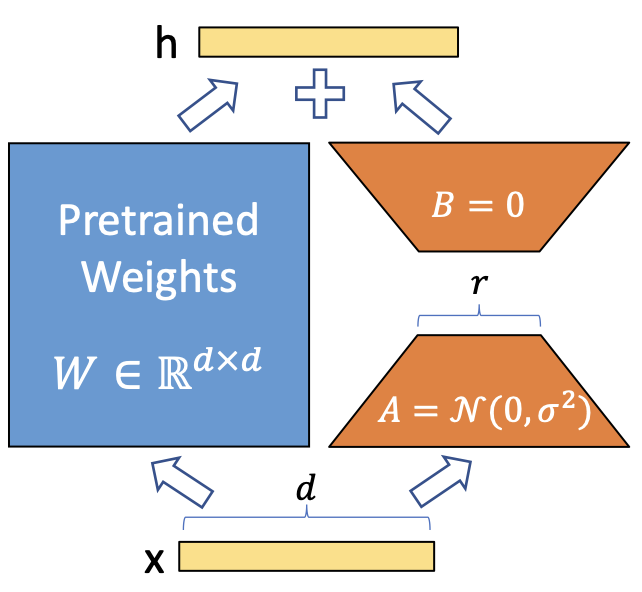
\includegraphics[width=0.22\textwidth]{Images/peft.png}
    \caption{Abstraction of LoRA from \citeauthor{hu2022lora} \cite{hu2022lora}.}
    \label{fig:lora}
\end{figure}

\section{Methodology}
\label{sec:approach}
In this study, the performance of a pre-optimized BERT model versus this BERT model fine-tuned using PEFT in relevancy labelling COVID-19 related document-query pairs is compared.
This comparison is performed using existing data and an existing BERT model pre-trained on predicting relevancy judgement scores of document-query pairs.
This pre-trained model is a Sentence-BERT model taken from Reimers and Gurevych \cite{reimers2019sentencebert}.
The specifically concerns the "msmarco-bert-base-dot-v5" model, a BERT model trained on data from the MS MARCO Passage Ranking dataset, optimized for representing documents as embeddings.
This model, alongside other Sentence-BERT models, are hosted online on Hugging Face under the Sentence Transformers package.
This package is also available as a Python package.

The dataset used to fine-tune the BERT and PEFT-BERT models is provided by Voorhees et al. \cite{voorhees2021trec} and is called the TREC-COVID dataset.
The TREC-COVID dataset is a collection of documents, queries, and relevancy judgements on the topic of COVID-19 and the pandemic that followed it.
The document collection consists of publications made during to the COVID-19 pandemic that are about COVID-19 and prior publications about other corona viruses.
The collection of queries was formulated by the bio-medically trained organizers of the TREC-COVID dataset.
The queries included in the dataset were inspired by common questions that were asked on social media.
The collection of relevancy judgements was made by a group of medical students from the Oregon Health and Science University and the organizers of TREC-COVID.
Professional indexers from the National Library of Medicine then assessed these relevancy judgements.
For the relevancy judgements, there are 3 levels of relevancy: "Not Relevant", "Partially Relevant", and "Relevant".
The TREC-COVID dataset was incorporated into the BEIR collection of IR evaluation datasets by Thakur et al. \cite{thakur2021beir}.
The version of TREC-COVID incorporated into BEIR was used for our research.
The BEIR collection is hosted on Hugging Face.

Both the BERT and PEFT BERT models were trained and evaluated on the TREC-COVID dataset.
In order for the pre-trained model to predict relevancy judgement scores, a dense linear layer was added at the end of the model's architecture that maps the pre-trained model's embeddings to the relevancy judgement scores.
This final dense linear layer was then trained.
While the additional dense linear layer was trained, the PEFT BERT model was further fine-tuned using LoRA, while the BERT model was not.
Both models were then evaluated on data from the TREC-COVID dataset: given a document and a query, the model should predict the relevancy judgement score of the document-query pair.

\section{Experimental Setup}
Our approach was implemented using the Python programming language.
The SentenceTransformers \cite{reimers2019sentencebert} package was used to retrieve the pre-trained BERT model.
The PyTorch and SentenceTransformer packages were used to alter and fine-tune the pre-trained BERT model.
HuggingFace's Datasets \cite{lhoest2021datasets} and PEFT \cite{huggingface2023peft} packages were used to retrieve the BEIR collection and to perform PEFT using LoRA respectively.
Additionally, the TensorBoard \footnote{https://github.com/tensorflow/tensorboard} package allowed us to visualize the training process of the models.
The code developed for our research can be found in a public GitHub repository (see appendix \ref{appendix:code}).

The TREC-COVID dataset was extracted from the BEIR collection.
Features from the TREC-COVID dataset besides the document titles, documents, queries, and relevancy judgement scores were dropped.
This resulted in a dataset of document-query pairs and their relevancy judgement score.
A total of 187.695 document-query pairs are included in this dataset.
An overview of the data distribution of the dataset is given in table \ref{tab:dataset_qrel_distribution}.

\begin{table}
    \centering
    \caption{Distribution of Relevancy Judgement Scores for the Unbalanced Pre-processed Document-Query Dataset}
    \label{tab:dataset_qrel_distribution}
    \begin{tabular}{c c c c}
    \toprule
    \textbf{Relevancy Score} & \textbf{Relevancy Level} & \textbf{Count} & \textbf{Share} \\
    \midrule
    0 & Not Relevant & 117.346 & 62.52\%\\
    1 & Partially Relevant & 29.798 & 15.88\%\\
    2 & Relevant & 40.545 & 21.6\%\\
    \bottomrule
    \end{tabular}
\end{table}

In addition to the document itself, BEIR's TREC-COVID dataset contains a title for every document. 
If such a title was present, we prepended it to the document string and processed this concatenation as the document.
We dropped data points with missing documents, queries, and/or relevancy judgement scores.
Invalid relevancy judgement scores, like -1, which in total occurred 3 times, were also excluded.

After this pre-processing, the dataset was split into train, validation, and test sets.
We assumed a split of 60\% train, 20\% validation, and 20\% test.
The data was randomly shuffled prior to splitting. We used a random state for PyTorch, NumPy and Pythons internal Random module to ensure every model was trained with the same samples.
Because the document-query pairs are are related in a many-to-many relationship, we applied extra pre-processing steps. Firstly, this involved making sets of all distinct document-ids and query-ids, and then allocate them in the train, validation and tests sets accordingly. Secondly, and extra check is done in the pre-processing pipeline to make sure no queries or documents overlap between sets. The downside of this pre-processing step, is that many document-query pairs in the dataset had to be dropped, decreasing the amount of usable data substantially. 
Table \ref{tab:train_val_test_spilt} shows the amount of document-query pairs in each split set.

\begin{table}[]
\caption{Distribution of Relevancy Judgement Scores for the unbalanced train, validation and test set}
\label{tab:train_val_test_spilt}
\begin{tabular}{c c c c}
\hline
\textbf{Split}                       & \textbf{Relevancy Score} & \textbf{Count} & \textbf{Share} \\ \hline
\multirow{3}{*}{Train}      & 0               & 41.270 & 63.5\%  \\ \cline{2-4} 
                            & 1               & 9.486  & 14.6\%  \\ \cline{2-4} 
                            & 2               & 14.238 & 21.9\%  \\ \cline{2-4} 
                       & \textbf{Total}               & \textbf{64.994} & \textbf{100\%}   \\ \hline
\multirow{3}{*}{Validation} & 0               & 5.166  & 63.8\%  \\ \cline{2-4} 
                            & 1               & 1.186  & 14.6\%  \\ \cline{2-4} 
                            & 2               & 1.751  & 21.6\%  \\ \cline{2-4} 
                       & \textbf{Total}               & \textbf{8.103}  & \textbf{100\%}   \\ \hline
\multirow{3}{*}{Test}       & 0               & 4.705  & 60.2\%  \\ \cline{2-4} 
                            & 1               & 1.427  & 18.3\%  \\ \cline{2-4} 
                            & 2               & 1.685  & 21.6\%  \\ \cline{2-4} 
                       & \textbf{Total}               & \textbf{7.817}  & \textbf{100\%}   \\ \hline
\end{tabular}
\end{table}

As table \ref{tab:dataset_qrel_distribution} and table \ref{tab:train_val_test_spilt} show, the pre-processed document-query dataset was quite unevenly distributed.
We expected that this may have a negative effect on the ability of a model to train on the data.
Because of this, we implemented a data rebalancing procedure that attempts to balance the distribution of relevancy judgement scores across the train, validation, and test sets, while adhering to the rule that no document or query data must be leaked to another set.
This was done by identifying the class distribution for all 3 sets, calculating where in these sets certain classes are over- or underrepresented, and moving a set of document-query pairs from one set to another. We used this strategy iteratively because moving document-query pairs from a set can free up space for another document-query pair to move. Every iteration, some entries of overbalanced classes in sets that contain most of the overbalanced class, are deducted to free up space for class balancing. 
This class balancing procedure resulted in train, validation, and test sets with a more even class distribution. The consequence of class balancing is that the dataset sizes are further reduced. The number of document-query pairs in this balanced split are shown in table \ref{tab:train_val_test_spilt_balanced}

\begin{table}[]
\caption{Distribution of Relevancy Judgement Scores for the balanced train, validation and test set}
\label{tab:train_val_test_spilt_balanced}
\begin{tabular}{c c c c}
\hline
\textbf{Split}                       & \textbf{Relevancy Score} & \textbf{Count} & \textbf{Share} \\ \hline
\multirow{3}{*}{Train}      & 0               & 10.153 & 34.8\%  \\ \cline{2-4} 
                            & 1               & 9.706  & 33.3\%  \\ \cline{2-4} 
                            & 2               & 9.277  & 31.8\%  \\ \cline{2-4} 
                            & \textbf{Total}           & \textbf{29.136} & \textbf{100\%}   \\ \hline
\multirow{3}{*}{Validation} & 0               & 1.068  & 33.3\%  \\ \cline{2-4} 
                            & 1               & 1.069  & 33.3\%  \\ \cline{2-4} 
                            & 2               & 1.069  & 33.3\%  \\ \cline{2-4} 
                            & \textbf{Total}           & \textbf{3.206}  & \textbf{100\%}   \\ \hline
\multirow{3}{*}{Test}       & 0               & 940   & 37.9\%  \\ \cline{2-4} 
                            & 1               & 712   & 28.7\%  \\ \cline{2-4} 
                            & 2               & 828   & 33.4\%  \\ \cline{2-4} 
                            & \textbf{Total}           & \textbf{2.480}  & \textbf{100\%}   \\ \hline
\end{tabular}
\end{table}

A variety of hyperparameters were used in the training of BERT and PEFT BERT, specific combinations of which we tried out are given in table \ref{tab:experimental_runs_val} and \ref{tab:experimental_runs_test}.
We used learning rates of 1e-4 and 1e-5 alongside a Softmax Loss function.
We trained models for 1 to 2 epochs on an unbalanced dataset, while training for 1 to 5 epochs on a balanced dataset.
We applied a dropout of 10\% during training on the final dense layer. All models were trained with a batch size of 32. 
Hyperparameters for LoRA include $r$ and $\alpha$. 
They were both set to 4 or 16, where $r$ stands for the rank of LoRA's $A$ and $B$ matrices and $\alpha$ was set to the same value as the rank.
Two scenarios were evaluated: one without class balancing, and one with class balancing which has fewer samples.

Model performance was evaluated using confusion matrices that describe the classification accuracy across the different relevancy judgement scores.
The F1-score was calculated for each class label to provide a weighted measure of precision and recall.
The weighted precision and weighted recall were also provided separately.
We also report the training time, and the amount of parameters fine-tuned during training, which provides insights into the computational efficiency of the models. 
To get insight into the efficiency of LoRA, we also fine-tune the full BERT model without any frozen trainable parameters. 
Because this costs a significant amount of time, we only train the BERT model with one set of parameters and with the balanced dataset, as the balanced dataset is significantly smaller. 
All training and evaluation was done using a Nvidia GeForce RTX 3060 GPU with 12 GB of memory.

\section{Results}
In table \ref{tab:experimental_runs_test}, the evaluation metrics of the different fine-tuned models are shown. The best performing BERT models and the best performing PEFT BERT models are highlighted in bold.
The best performing model is the model that was fine-tuned using PEFT, has a learning rate of 1e-4, and an $r$ and $\alpha$ of 16. 
We report a weighted F1-score of 0.520. This model was trained without balanced classes in the training set. 
The best BERT model without using PEFT trained without balanced classes has an F1-score of 0.305, which is substantially lower. 
When using balanced classes, the best performing BERT model without using PEFT has a F1-score of 0.367. 
This F1-score is lower than the F1-score of the PEFT model trained on the same balanced data: 0.389.


\begin{table*}[h]
\centering
\caption{Summary of Configurations and Weighted Performance Metrics for Different BERT Model Variants in Experimental Runs on Test Set. BERT and PEFT-BERT models with highest evaluation metrics are in bold.}
\label{tab:experimental_runs_test}
\begin{tabular}{c c c c c c c c c}
\toprule
\textbf{Model} & \textbf{Learning Rate} & \textbf{Epochs} & \textbf{LoRA Config} & \textbf{Frozen Params} & \textbf{Training time} & \textbf{Recall} & \textbf{Precision} & \textbf{F1-Score} \\ 
\midrule
BERT & 1e-4 & 1 & - & 100\% & 1.219hr & 0.194 & 0.567 & 0.289 \\ 
BERT & 1e-4 & 2 & - & 100\%  & 3.153hr & 0.196 & 0.567 & 0.291 \\
\textbf{BERT} & \textbf{1e-5} & \textbf{1} & \textbf{-} & \textbf{100\%} & \textbf{1.219hr} & \textbf{0.223} & \textbf{0.483} &  \textbf{0.305} \\ 
BERT & 1e-5 & 2 & - & 100\%  & 2.551hr & 0.217 & 0.442 & 0.291 \\ 
PEFT BERT & 1e-4 & 1 & r: 16, $\alpha$: 16 & 99.45\% & 1.278hr & 0.452 & 0.429 & 0.440\\ 
PEFT BERT & 1e-4 & 1 & r: 4, $\alpha$: 4 & 99.85\% & 1.277hr & 0.423 & 0.408 & 0.415 \\ 
\textbf{PEFT BERT} & \textbf{1e-4} & \textbf{2} & \textbf{r: 16, $\alpha$: 16} & \textbf{99.45\%} & \textbf{2.749 hr} & \textbf{0.576} & \textbf{0.443} &  \textbf{0.501} \\ 
PEFT BERT & 1e-4 & 2 & r: 4, $\alpha$: 4 & 99.85\% & 2.774hr & 0.194 & 0.567 &  0.289 \\ 
PEFT BERT & 1e-5 & 1 & r: 16, $\alpha$: 16 & 99.45\%  & 1.278hr & 0.488 & 0.464 & 0.476 \\ 
PEFT BERT & 1e-5 & 1 & r: 4, $\alpha$: 4 & 99.85\%  & 1.293hr & 0.263 & 0.497 & 0.344 \\ 
PEFT BERT & 1e-5 & 2 & r: 16, $\alpha$: 16 & 99.45\% & 2.689hr & 0.602 & 0.362 &  0.452 \\ 
\midrule
\multicolumn{8}{c}{\textit{Runs with Class Balancing:}} \\
\midrule
\textbf{BERT} & \textbf{1e-5} & \textbf{2} & - & \textbf{100\%} & \textbf{39.27min} & \textbf{0.337} & \textbf{0.403} &\textbf{ 0.367} \\ 
BERT & 1e-5 & 5 & - & 100\%  & 2.713hr & 0.288 & 0.399 & 0.335 \\ 
BERT & 1e-5 & 1 & - & 0\%  & 7.705hr & 0.285 & 0.492 & 0.361 \\ 
PEFT BERT & 1e-5 & 2 & r: 16, $\alpha$: 16 & 99.45\% & 41.18min & 0.288 & 0.399 &  0.335 \\
\textbf{PEFT BERT} & \textbf{1e-5} & \textbf{5} & \textbf{r: 16, $\alpha$: 16} & \textbf{99.45\%} & \textbf{1.867hr} & \textbf{0.383} & \textbf{0.395} & \textbf{0.389}\\
\bottomrule
\end{tabular}
\end{table*}

Validation and train scores can be found in table \ref{tab:experimental_runs_val} and table \ref{tab:experimental_runs_train} of appendix \ref{appendix:val-scores}. 
When comparing the test scores of the 2 best BERT models and the 2 best PEFT models to their train scores, we notice some overfitting for all four models. 
The model that shows the biggest difference between the train and test scores is the BERT model that was trained with balanced classes. 
Here we see that the train F1-score is 0.103 higher than the test F1-score. 
We notice that both models trained with balanced classes show a somewhat bigger difference between the train and test scores. 
This could be explained by the fact that these models were trained with a significantly smaller dataset, therefore needing more epochs for training.

What is also clear from table \ref{tab:experimental_runs_test} is that there is very little difference in training time between the BERT models and the PEFT BERT models. 
For both models, a very low number of parameters was trained. 
Therefore, the training times are much smaller compared to fine-tuning all trainable parameters of BERT. 
We see a large difference in training time between the PEFT BERT model and the fully fine-tuned BERT model. 
One epoch using PEFT on BERT takes about 20 minutes, while fine-tuning all parameters of BERT on the same dataset takes almost 8 hours.

\begin{table}[H]
\caption{Confusion Matrices for (PEFT) BERT Models on Test Set}
\centering 
\begin{minipage}{.45\linewidth}
\label{tab:bertConf}
\begin{tabular}{cc|c|c|c|p{1cm}|}
&\multicolumn{1}{c}{}&\multicolumn{3}{c}{\textbf{Predicted}}\\
&\multicolumn{1}{c}{}&\multicolumn{1}{c}{\textbf{0}}
&\multicolumn{1}{c}{\textbf{1}}
&\multicolumn{1}{c}{\textbf{2}}
&\multicolumn{1}{c}{\textbf{Share}}\\
\cline{3-6}
\multicolumn{1}{c}{\multirow{3}{*}{\rotatebox{90}{\textbf{Actual}}}}
&\textbf{0} &10 &0 &930&37.5\%\\
\cline{3-6}
&\textbf{1} &1 &0 &711&28.7\%\\
\cline{3-6}
&\textbf{2} &2 &0 &826&33.4\%\\
\cline{3-6}
\end{tabular}
\centering
\newline
\textbf{BERT Model}
\end{minipage}%
\begin{minipage}{.45\linewidth}
\label{tab:peftBertConv}
\begin{tabular}{cc|c|c|c|p{1cm}|}
&\multicolumn{1}{c}{}&\multicolumn{3}{c}{\textbf{Predicted}}\\
&\multicolumn{1}{c}{}&\multicolumn{1}{c}{\textbf{0}}
&\multicolumn{1}{c}{\textbf{1}}
&\multicolumn{1}{c}{\textbf{2}}
&\multicolumn{1}{c}{\textbf{Share}}\\
\cline{3-6}
\multicolumn{1}{c}{\multirow{3}{*}{\rotatebox{90}{\textbf{Actual}}}}
&\textbf{0} &4357 &26 &322 &60.2\%\\
\cline{3-6}
&\textbf{1} &1315 &5 &107 &18.3\%\\
\cline{3-6}
&\textbf{2} &1540 &4 &141 &21.6\%\\
\cline{3-6}
\end{tabular}
\centering
\newline
\textbf{PEFT BERT Model}
\end{minipage}
\end{table}


In the provided confusion matrices (table \ref{tab:bertConf}), the PEFT BERT model outperforms the BERT model, particularly in distinguishing different relevancy judgement scores. 
The PEFT BERT model accurately predicts 4357 instances for relevancy label 0. 
Even though it has a share of 60.2\% for label 0, it is still far outperforming the BERT model, which only correctly identifies 10 instances (share 37.5\%). 
Relevancy label 1 is difficult for both models, with the BERT model failing to correctly classify any instances in this category and the PEFT BERT model managing only 5 correct predictions, indicating some difficulty in this area. 
For relevancy label 2, the BERT model has a slightly higher accuracy with 826 correct predictions, compared to the PEFT BERT model's 141. 
However, we should be cautious of this finding, because the BERT model's dataset has a greater percentage of relevancy label 2, and BERT predicts relevancy label 2 when it is actually 0 or 1, in almost all cases. 

\section{Discussion and Outlook}
The results suggest, despite not implementing class balancing, the PEFT BERT model outperforms the BERT model significantly. This implies that model architecture and training parameters, or inherent efficiencies in the PEFT BERT model, could play a critical role in its elevated predictive accuracy.

In analyzing the results for the BERT and PEFT BERT models (table \ref{tab:bertConf}), two main limitations stand out due to the nature of the dataset and the models' behavior.
First, there is a clear trend in which the BERT model mostly predicts one specific class - relevancy label 2. 
This could imply that the model is not able to generalize enough, causing it to be unable to accurately recognise the other relevancy judgement scores. 
The PEFT BERT model shows a similar tendency, although to a lesser extent, implying that it may generalize better. 
Second, the class balancing process in the dataset presents a difficult situation. 
Because many document-query pairs in the original dataset overlap, removing duplicates to avoid repetition across training, testing, and validation sets results in significant data loss. 
This step could have an impact on the dataset's representativeness. 
In most real-world scenarios, the majority of documents are irrelevant (label 0), making this imbalance appear less problematic. 
However, it is important to remember that, despite being uncommon, finding relevant documents is often more important. 
As shown in table \ref{tab:experimental_runs_test}, we chose to not choose either of these arguments, and set class balancing as a hyperparameter. 
Table \ref{tab:experimental_runs_test} shows that introducing class balancing increases BERT's F1-score significantly. 
As previously stated, BERT assigns a single label to each entry. 
Because this version of BERT is trained on a balanced dataset, the model learned to generalise slightly better, more evenly balancing the recall and precision, causing the F1-score to rise. 
PEFT BERT, however, does not share this performance boost when trained on a balanced dataset. 
This could mean that the extra size of the unbalanced dataset is impactful on improving performance, compared to class balancing with fewer entries. 
As a result, we can conclude that using PEFT for BERT classifiers reduces the susceptibility to class imbalance.

The relevancy judgement score 1 appears to be a problem for both the BERT and PEFT BERT models. 
This score is between 0 and 2, making it similar to both other labels and thus more difficult to classify. 
Based on this result, we can conclude that the BERT and PEFT BERT models have not yet been sufficiently optimised to classify three labels. 
We can also conclude from the confusion matrices in table \ref{tab:bertConf} that PEFT BERT might do better in binary classifications.  

\subsection{Related Work} 
Hu et al.\cite{hu2022lora} state that applying PEFT to BERT-based models with LoRA improves generalizability, accuracy, and resource efficiency. 
In table \ref{tab:experimental_runs_test} we see similarities. The BERT model requires approximately 7.7 hours to train the full set of parameters, whereas PEFT BERT ($r$: 16 $\alpha$: 16) reduces this to 21 minutes per epoch while increasing generalizability and the F1-score. 

\citeauthor{pfeiffer2020} \cite{pfeiffer2020} state that LoRA is well suited for domain adaptation and quick task switching in BERT-based models. 
Despite the fact that our results show that PEFT BERT significantly increases training time and improves performance when compared to a basic BERT-based model, these results do not compare to other domain adaptation methods. 
As a result, we are unable to validate the findings of \citeauthor{pfeiffer2020}. 

\subsection{Future Work}
Taking the results of our research into account, we suggest some points of potential further research.
We chose to adapt a pre-trained BERT model to data of the COVID-19 pandemic.
Further research may show whether PEFT can be used to fine-tune BERT to improve performance on other unseen domains.
Apart from this, we have only considered the use of LoRA as a PEFT method.
However, the application of other PEFT methods following similar methodologies might prove fruitful.
For example, there exist other PEFT methods that build upon LoRA, such as AdaLoRA \cite{zhang2023adaptive}, which attempts to reduce required computation further by only fine-tuning weights that provide the most information. This method may increase computational efficiency even further. 
Additionally, future work could focus on a retrieval use-case instead of a classification use-case as researched in this paper.

\subsection{Conclusion}
We conclude that fine-tuning (PEFT) BERT to out-of-domain datasets is not an easy task. 
Both models, BERT and PEFT BERT, were not able to achieve significant performance. 
We can conclude however, that fine-tuning BERT using PEFT, specifically LoRA, performs better than standalone BERT with frozen parameters during training. Therefore, we recommend doing more research towards the use of LoRA for information retrieval.
\bibliographystyle{ACM-Reference-Format}
\def\bibfont{\small} % comment this line for a smaller fontsize
\bibliography{refs.bib} 

\pagebreak

\onecolumn
\begin{appendices}
\setcounter{table}{0}

\section{\label{appendix:code}Code}
The following link leads to the GitHub repository containing the code used in this research: 
\hyperlink{https://github.com/JulianRodd/projectInformationRetrieval}{https://github.com/JulianRodd/projectInformationRetrieval}

\section{\label{appendix:val-scores}Evaluation metrics}

\begin{table}[h]
\caption{Summary of Configurations and Weighted Performance Metrics for Best BERT Model Variants in Experimental Runs on Validation Sets}
\label{tab:experimental_runs_val}
% \resizebox{\textwidth}{!}{%
% \begin{tabular}{@{}p{2cm}p{1.5cm}p{1.2cm}p{1.5cm}p{1.5cm}p{1.2cm}p{1.5cm}p{1.5cm}p{1.5cm}{1.5cm}@{}}
\begin{tabular}{c c c c c c c}
\toprule
\textbf{Model} & \textbf{Learning Rate} & \textbf{Epochs} & \textbf{LoRA Config} & \textbf{Recall} & \textbf{Precision} & \textbf{F1-Score} \\ 
\midrule
BERT & 1e-5 & 1 & - & 0.223 & 0.462 & 0.301\\ 
PEFT BERT & 1e-4 & 2 & r: 16, $\alpha$: 16 & 0.604 & 0.450 & 0.516 \\ 
\midrule
\multicolumn{7}{c}{\textit{Runs with Class Balancing:}} \\
\midrule
BERT & 1e-5 & 2 & - & 0.334 & 0.213 & 0.260\\ 
PEFT BERT & 1e-5 & 5 & r: 16, $\alpha$: 16 & 0.337 & 0.377 & 0.356\\
\bottomrule
\end{tabular}
% }
\end{table}

\begin{table}[h]
\caption{Summary of Configurations and Weighted Performance Metrics for Best BERT Model Variants in Experimental Runs on Train Sets}
\label{tab:experimental_runs_train}
% \resizebox{\textwidth}{!}{%
% \begin{tabular}{@{}p{2cm}p{1.5cm}p{1.2cm}p{1.5cm}p{1.5cm}p{1.2cm}p{1.5cm}p{1.5cm}p{1.5cm}{1.5cm}@{}}
\begin{tabular}{c c c c c c c}
\toprule
\textbf{Model} & \textbf{Learning Rate} & \textbf{Epochs} & \textbf{LoRA Config} & \textbf{Recall} & \textbf{Precision} & \textbf{F1-Score} \\ 
\midrule
BERT & 1e-5 & 1 & - & 0.225 & 0.491 & 0.309 \\ 
PEFT BERT & 1e-4 & 2 & r: 16, $\alpha$: 16 & 0.610 & 0.475 & 0.534 \\ 
\midrule
\multicolumn{7}{c}{\textit{Runs with Class Balancing:}} \\
\midrule
BERT & 1e-5 & 2 & - & 0.319 & 0.226 & 0.264 \\ 
PEFT BERT & 1e-5 & 5 & r: 16, $\alpha$: 16 & 0.346 & 0.324 & 0.335 \\
\bottomrule
\end{tabular}
% }
\end{table}

\end{appendices}

\end{document}

\end{document}
